\documentclass[10pt,twocolumn]{article}
\usepackage[a4paper,margin=1.8cm,columnsep=0.6cm]{geometry}
\usepackage{mathptmx}
\usepackage{amsmath,graphicx,booktabs,caption,subcaption,url,enumitem}
\usepackage[hidelinks]{hyperref}
\usepackage[numbers,sort]{natbib}
\usepackage[compact]{titlesec}
\titleformat{\section}{\normalfont\large\bfseries}{\thesection.}{0.5em}{}
\titleformat{\subsection}{\normalfont\normalsize\bfseries}{\thesubsection}{0.5em}{}
\titleformat{\paragraph}[runin]{\normalfont\normalsize\itshape}{}{0em}{}
% generated by scripts/collect_numbers.py from results/numbers.json; do not edit
\newcommand{\humanKappa}{\ensuremath{0.002}}
\newcommand{\humanLamRhombus}{\ensuremath{0.022}}
\newcommand{\humanLamGrating}{\ensuremath{0.57}}
\newcommand{\humanLamPlaid}{\ensuremath{1.2}}
\newcommand{\humanThinLowErr}{\ensuremath{33.2}}
\newcommand{\humanFatLowErr}{\ensuremath{15.5}}
\newcommand{\humanThinHighErr}{\ensuremath{1.9}}
\newcommand{\humanFatHighErr}{\ensuremath{0.24}}
\newcommand{\humanLamFit}{\ensuremath{0.96}}
\newcommand{\humanLamFitLo}{\ensuremath{0.22}}
\newcommand{\humanLamFitHi}{\ensuremath{2.0}}
\newcommand{\humanFitRSS}{\ensuremath{596}}
\newcommand{\humanFitRMSE}{\ensuremath{10.0}}
\newcommand{\humanFitMaxResid}{\ensuremath{19.5}}
\newcommand{\humanFitResidAtThirty}{\ensuremath{-19.5}}
\newcommand{\humanNDigitized}{\ensuremath{6}}
\newcommand{\humanRecoveryMaxRelErr}{\ensuremath{0.036}}
\newcommand{\humanGratingRelSpeedFortyAtTenth}{\ensuremath{0.45}}
\newcommand{\humanGratingRelSpeedSeventyAtTenth}{\ensuremath{0.71}}
\newcommand{\humanPlaidTwoLowDir}{\ensuremath{52.3}}
\newcommand{\humanPlaidTwoHighDir}{\ensuremath{4.6}}
\newcommand{\humanPlaidOneLowDir}{\ensuremath{7.3\times 10^{-17}}}
\newcommand{\humanPlaidTwoVA}{\ensuremath{57.1}}
\newcommand{\humanPlaidBiasLowMax}{\ensuremath{44.7}}
\newcommand{\humanPlaidBiasHighMax}{\ensuremath{37.8}}
\newcommand{\paperRssNonpredictive}{\ensuremath{3.1}}
\newcommand{\paperRssFixed}{\ensuremath{0.99}}
\newcommand{\paperShiftFixed}{\ensuremath{10.3}}
\newcommand{\paperRssVelocity}{\ensuremath{0.89}}
\newcommand{\paperRssPredictive}{\ensuremath{0.15}}
\newcommand{\paperShiftPredictive}{\ensuremath{6.2}}
\newcommand{\paperKPredictive}{\ensuremath{5}}
\newcommand{\paperKVelocity}{\ensuremath{2}}
\newcommand{\paperNBL}{\ensuremath{97}}
\newcommand{\paperNOL}{\ensuremath{62}}
\newcommand{\paperLeadT}{\ensuremath{4.1}}
\newcommand{\paperLeadDf}{\ensuremath{97}}
\newcommand{\paperLeadR}{\ensuremath{0.38}}
\newcommand{\paperRssOccNonpredictive}{\ensuremath{4.4}}
\newcommand{\paperRssOccPredictive}{\ensuremath{0.41}}
\newcommand{\paperChgOMFAfterNonpredictive}{\ensuremath{0.047}}
\newcommand{\paperChgOMFAfterPredictive}{\ensuremath{3.4}}
\newcommand{\paperChgOMSAfterNonpredictive}{\ensuremath{0.29}}
\newcommand{\paperChgOMSAfterPredictive}{\ensuremath{0.47}}
\newcommand{\realNBats}{\ensuremath{4}}
\newcommand{\realNTrialsAll}{\ensuremath{657}}
\newcommand{\realNBL}{\ensuremath{94}}
\newcommand{\realNOL}{\ensuremath{62}}
\newcommand{\realNCatch}{\ensuremath{98}}
\newcommand{\realNBMF}{\ensuremath{74}}
\newcommand{\realNOMF}{\ensuremath{75}}
\newcommand{\realNBMS}{\ensuremath{62}}
\newcommand{\realNOMS}{\ensuremath{56}}
\newcommand{\realCallRateMedianHz}{\ensuremath{9.2}}
\newcommand{\realCallIntervalMedianMs}{\ensuremath{50.5}}
\newcommand{\realCallIntervalCV}{\ensuremath{0.77}}
\newcommand{\realLeadBins}{\ensuremath{73}}
\newcommand{\realLeadMeanDeg}{\ensuremath{8.0}}
\newcommand{\realLeadSigBins}{\ensuremath{42}}
\newcommand{\realLeadMinT}{\ensuremath{1.4}}
\newcommand{\realLeadMaxT}{\ensuremath{6.3}}
\newcommand{\realLeadMaxPBonf}{\ensuremath{1}}
\newcommand{\realLeadFirstSigMs}{\ensuremath{-660}}
\newcommand{\realLeadTrialT}{\ensuremath{5.6}}
\newcommand{\realLeadTrialP}{\ensuremath{2.2\times 10^{-7}}}
\newcommand{\realLeadTrialDf}{\ensuremath{93}}
\newcommand{\realLeadTrialR}{\ensuremath{0.50}}
\newcommand{\realRssNonpredictive}{\ensuremath{5.4}}
\newcommand{\realRssOccNonpredictive}{\ensuremath{8.3}}
\newcommand{\realShiftNonpredictive}{\ensuremath{0}}
\newcommand{\realRssFixed}{\ensuremath{0.61}}
\newcommand{\realRssOccFixed}{\ensuremath{0.57}}
\newcommand{\realShiftFixed}{\ensuremath{15.5}}
\newcommand{\realRssVelocity}{\ensuremath{2.1}}
\newcommand{\realRssOccVelocity}{\ensuremath{3.9}}
\newcommand{\realShiftVelocity}{\ensuremath{0}}
\newcommand{\realRssPredictive}{\ensuremath{0.19}}
\newcommand{\realRssOccPredictive}{\ensuremath{0.63}}
\newcommand{\realShiftPredictive}{\ensuremath{9.7}}
\newcommand{\realRssOursnoprior}{\ensuremath{0.19}}
\newcommand{\realRssOccOursnoprior}{\ensuremath{0.64}}
\newcommand{\realShiftOursnoprior}{\ensuremath{9.8}}
\newcommand{\realRssOurs}{\ensuremath{0.19}}
\newcommand{\realRssOccOurs}{\ensuremath{0.64}}
\newcommand{\realShiftOurs}{\ensuremath{9.8}}
\newcommand{\realKPredictive}{\ensuremath{5}}
\newcommand{\realKVelocity}{\ensuremath{2}}
\newcommand{\realKOurs}{\ensuremath{5}}
\newcommand{\realLamOurs}{\ensuremath{0}}
\newcommand{\realCvNonpredictive}{\ensuremath{32.3}}
\newcommand{\realCvFixed}{\ensuremath{15.0}}
\newcommand{\realCvVelocity}{\ensuremath{16.7}}
\newcommand{\realCvPredictive}{\ensuremath{11.2}}
\newcommand{\realCvOursnoprior}{\ensuremath{11.1}}
\newcommand{\realCvOurs}{\ensuremath{11.7}}
\newcommand{\realCvOursLamChoices}{30000, 300, 0, 0}
\newcommand{\realCvOursLamZeroCount}{\ensuremath{2}}
\newcommand{\realPPredictiveVsNonpredictive}{\ensuremath{6.0\times 10^{-5}}}
\newcommand{\realRPredictiveVsNonpredictive}{\ensuremath{-0.54}}
\newcommand{\realPPredictiveVsVelocity}{\ensuremath{0.48}}
\newcommand{\realRPredictiveVsVelocity}{\ensuremath{-0.088}}
\newcommand{\realPPredictiveVsFixed}{\ensuremath{1.8\times 10^{-5}}}
\newcommand{\realRPredictiveVsFixed}{\ensuremath{-0.58}}
\newcommand{\realPOursVsPredictive}{\ensuremath{0.033}}
\newcommand{\realROursVsPredictive}{\ensuremath{0.30}}
\newcommand{\realPOursVsOursnoprior}{\ensuremath{0.013}}
\newcommand{\realROursVsOursnoprior}{\ensuremath{0.51}}
\newcommand{\realChangeOursBeatsPredCount}{\ensuremath{5}}
\newcommand{\realChangeNonpredBeatsPredAfterOccl}{\ensuremath{1}}
\newcommand{\realChgBMFBeforeNonpredictive}{\ensuremath{14.6}}
\newcommand{\realChgBMFBeforePredictive}{\ensuremath{3.7}}
\newcommand{\realChgBMFBeforeOurs}{\ensuremath{3.4}}
\newcommand{\realChgBMFAfterNonpredictive}{\ensuremath{1.6}}
\newcommand{\realChgBMFAfterPredictive}{\ensuremath{1.1}}
\newcommand{\realChgBMFAfterOurs}{\ensuremath{0.64}}
\newcommand{\realChgOMFBeforeNonpredictive}{\ensuremath{33.9}}
\newcommand{\realChgOMFBeforePredictive}{\ensuremath{5.1}}
\newcommand{\realChgOMFBeforeOurs}{\ensuremath{5.4}}
\newcommand{\realChgOMFAfterNonpredictive}{\ensuremath{0.13}}
\newcommand{\realChgOMFAfterPredictive}{\ensuremath{3.2}}
\newcommand{\realChgOMFAfterOurs}{\ensuremath{1.3}}
\newcommand{\realChgBMSBeforeNonpredictive}{\ensuremath{16.0}}
\newcommand{\realChgBMSBeforePredictive}{\ensuremath{3.9}}
\newcommand{\realChgBMSBeforeOurs}{\ensuremath{3.7}}
\newcommand{\realChgBMSAfterNonpredictive}{\ensuremath{5.0}}
\newcommand{\realChgBMSAfterPredictive}{\ensuremath{0.40}}
\newcommand{\realChgBMSAfterOurs}{\ensuremath{0.46}}
\newcommand{\realChgOMSBeforeNonpredictive}{\ensuremath{44.2}}
\newcommand{\realChgOMSBeforePredictive}{\ensuremath{14.1}}
\newcommand{\realChgOMSBeforeOurs}{\ensuremath{14.2}}
\newcommand{\realChgOMSAfterNonpredictive}{\ensuremath{1.3}}
\newcommand{\realChgOMSAfterPredictive}{\ensuremath{0.70}}
\newcommand{\realChgOMSAfterOurs}{\ensuremath{0.46}}
\newcommand{\simNTrialsPerCell}{\ensuremath{500}}
\newcommand{\simNTrialsCurves}{\ensuremath{200}}
\newcommand{\simBaseRateHz}{\ensuremath{20}}
\newcommand{\simBaseNoiseMm}{\ensuremath{10}}
\newcommand{\simTolDeg}{\ensuremath{5}}
\newcommand{\simSigmaP}{\ensuremath{1}}
\newcommand{\simNCells}{\ensuremath{26}}
\newcommand{\simNTests}{\ensuremath{102}}
\newcommand{\simCoverage}{\ensuremath{0.95}}
\newcommand{\simSteadyRmsOurs}{\ensuremath{1.3}}
\newcommand{\simSteadyRmsNonpred}{\ensuremath{5.7}}
\newcommand{\simSteadyRmsOursLo}{\ensuremath{1.3}}
\newcommand{\simSteadyRmsOursHi}{\ensuremath{1.4}}
\newcommand{\simSteadyRmsNonpredLo}{\ensuremath{5.6}}
\newcommand{\simSteadyRmsNonpredHi}{\ensuremath{5.9}}
\newcommand{\simSteadyOffOurs}{\ensuremath{5.5}}
\newcommand{\simSteadyOffNonpred}{\ensuremath{197}}
\newcommand{\simHTwoP}{\ensuremath{1.3\times 10^{-81}}}
\newcommand{\simHTwoR}{\ensuremath{-1}}
\newcommand{\simHiddenFastExitOurs}{\ensuremath{6.5}}
\newcommand{\simHiddenFastExitNonpred}{\ensuremath{11.9}}
\newcommand{\simHiddenFastRecOurs}{\ensuremath{195}}
\newcommand{\simHiddenFastRecNonpred}{\ensuremath{253}}
\newcommand{\simHThreeFastP}{\ensuremath{1.3\times 10^{-81}}}
\newcommand{\simHThreeFastR}{\ensuremath{-1}}
\newcommand{\simHiddenSlowExitOurs}{\ensuremath{52.3}}
\newcommand{\simHiddenSlowExitNonpred}{\ensuremath{11.6}}
\newcommand{\simHiddenSlowRecOurs}{\ensuremath{38.6}}
\newcommand{\simHiddenSlowRecNonpred}{\ensuremath{38.6}}
\newcommand{\simHThreeSlowP}{\ensuremath{1.3\times 10^{-81}}}
\newcommand{\simHThreeSlowR}{\ensuremath{1.00}}
\newcommand{\simStdExitOurs}{\ensuremath{1.6}}
\newcommand{\simStdExitNonpred}{\ensuremath{11.7}}
\newcommand{\simNoiseTwoGain}{\ensuremath{8.3\times 10^{-5}}}
\newcommand{\simNoiseTwoR}{\ensuremath{-0.059}}
\newcommand{\simNoiseFiveGain}{\ensuremath{0.003}}
\newcommand{\simNoiseFiveR}{\ensuremath{-0.13}}
\newcommand{\simNoiseOneZeroGain}{\ensuremath{0.010}}
\newcommand{\simNoiseOneZeroR}{\ensuremath{-0.095}}
\newcommand{\simNoiseTwoZeroGain}{\ensuremath{0.077}}
\newcommand{\simNoiseTwoZeroR}{\ensuremath{-0.22}}
\newcommand{\simNoiseFourZeroGain}{\ensuremath{0.53}}
\newcommand{\simNoiseFourZeroR}{\ensuremath{-0.44}}
\newcommand{\simNoiseEightZeroGain}{\ensuremath{2.6}}
\newcommand{\simNoiseEightZeroR}{\ensuremath{-0.72}}
\newcommand{\simPriorHelpsAt}{20, 40, 80}
\newcommand{\simPriorHurtsAt}{none}
\newcommand{\simPriorHelpsMin}{\ensuremath{20}}
\newcommand{\simOcclNineZeroExitOurs}{\ensuremath{0.75}}
\newcommand{\simOcclNineZeroExitNonpred}{\ensuremath{5.9}}
\newcommand{\simOcclOneEightZeroExitOurs}{\ensuremath{1.4}}
\newcommand{\simOcclOneEightZeroExitNonpred}{\ensuremath{11.9}}
\newcommand{\simOcclTwoSevenZeroExitOurs}{\ensuremath{2.4}}
\newcommand{\simOcclTwoSevenZeroExitNonpred}{\ensuremath{19.8}}
\newcommand{\simOcclThreeSixZeroExitOurs}{\ensuremath{4.2}}
\newcommand{\simOcclThreeSixZeroExitNonpred}{\ensuremath{30.6}}
\newcommand{\simRateFiveRmsOurs}{\ensuremath{5.4}}
\newcommand{\simRateFiveRmsNonpred}{\ensuremath{18.8}}
\newcommand{\simRateFourZeroRmsOurs}{\ensuremath{1.6}}
\newcommand{\simRateFourZeroRmsNonpred}{\ensuremath{5.2}}

\graphicspath{{../figures/}}
\captionsetup{font=small,labelfont=bf}
\setlength{\bibsep}{2pt}
\renewcommand{\topfraction}{0.95}\renewcommand{\dbltopfraction}{0.8}
\renewcommand{\textfraction}{0.05}\renewcommand{\floatpagefraction}{0.8}\renewcommand{\dblfloatpagefraction}{0.8}
\setcounter{dbltopnumber}{2}\setcounter{topnumber}{3}

\begin{document}
\twocolumn[{%
\begin{center}
{\LARGE\bfseries From Eye to Echo: one slow-motion prior for human\\[2pt] motion illusions and bat target tracking\par}
\vspace{10pt}
{\large Deep Buha\par}
{Roll No.\ 24110082\par}
{CG-501 Computation and Cognition, IIT Gandhinagar\par}
{20 November 2026\par}
\vspace{10pt}
\begin{minipage}{0.86\textwidth}
\small\textbf{Abstract.} Weiss, Simoncelli and Adelson (2002) explained several human motion illusions with one idea: measurements are noisy, and slow motion is more likely than fast. I rebuilt their model and reproduced the rhombus, grating and plaid illusions: a thin rhombus at 10\% contrast is seen \humanThinLowErr$^\circ$ away from its true direction, a fat one only \humanFatLowErr$^\circ$. With echoes in place of image measurements, the same formula becomes a line fit through recent echoes. In a simulation of the bat experiment of Salles et al.\ (2020), this line fit stayed within \simSteadyRmsOurs$^\circ$ (RMS) of a steadily moving target, against \simSteadyRmsNonpred$^\circ$ for aiming at the last echo, but it failed when the target slowed down while hidden. On real head-tracking data from \realNBats{} bats, models that predict fit much better than the last echo, but the slow-motion prior did not help: its best strength was zero.
\end{minipage}
\vspace{14pt}
\end{center}
}]

\section{Introduction}
\subsection{Background and rationale}
To act on a moving object, a brain has to estimate its speed and direction from noisy, incomplete measurements. A person looking at a moving edge sees only the motion across the edge, not along it (the aperture problem), and a faint edge gives weak evidence. A bat gets one position from each echo, and none while the target is behind an obstacle. This project asks whether one estimator, with one expectation (a prior), can describe both.

\subsection{Review of relevant literature}
Weiss et al.\ \cite{weiss2002} modelled the observer as a Bayesian estimator. The likelihood assumes that brightness stays the same as an object moves, plus Gaussian noise; the prior is a Gaussian centred on zero velocity, so slow speeds are more likely. With one free parameter, $\lambda=\sigma^2/\sigma_p^2$ (measurement noise over prior width), the model explains why faint thin rhombuses seem to move diagonally, why faint gratings look slower, and why type II plaids move toward the vector average. Stocker and Simoncelli \cite{stocker2005} later measured the prior from human data and found heavier tails than a Gaussian.

Salles, Diebold and Moss \cite{salles2020} trained four big brown bats to follow a target moving across a track, sometimes behind an occluder and sometimes with a sudden speed change. A model that estimates speed from the last five echoes and adds a fixed angle fitted the head direction better than pointing at the last echo (residual sum of squares, RSS, \paperRssPredictive{} vs \paperRssNonpredictive{} rad$^2$ \cite{salles2020si}). Their data and code are public \cite{sallesrepo}.

\begin{figure*}[!tp]
\centering
\begin{subfigure}{0.49\textwidth}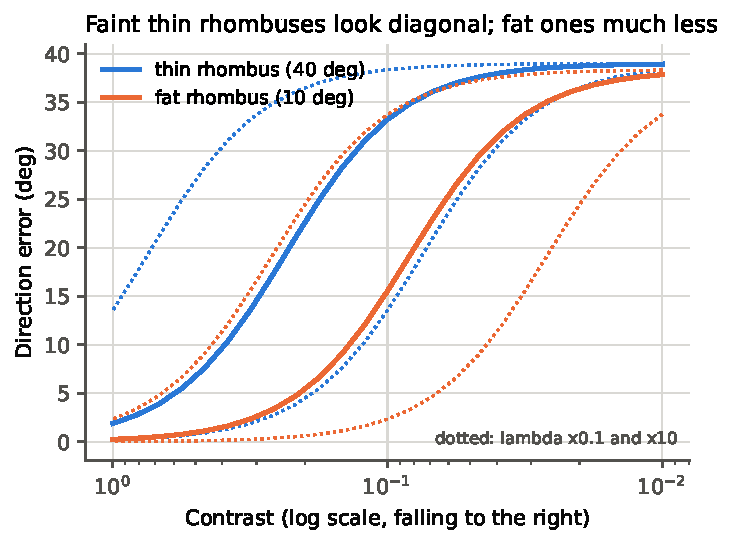
\includegraphics[width=\linewidth]{fig01_rhombus_contrast.pdf}\caption{}\end{subfigure}
\begin{subfigure}{0.49\textwidth}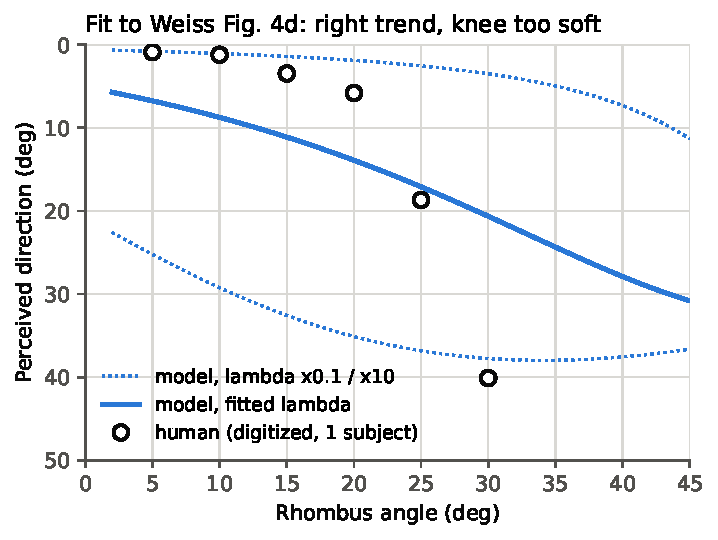
\includegraphics[width=\linewidth]{fig02_rhombus_angle_fit.pdf}\caption{}\end{subfigure}
\caption{Rhombus. (a) Direction error vs contrast; dotted: $\lambda\times0.1$ and $\times10$. (b) Seen direction vs rhombus angle; circles: one subject (Weiss Fig.~4d); line: fitted model.}
\label{fig:human}
\end{figure*}
\begin{figure*}[!tp]
\centering
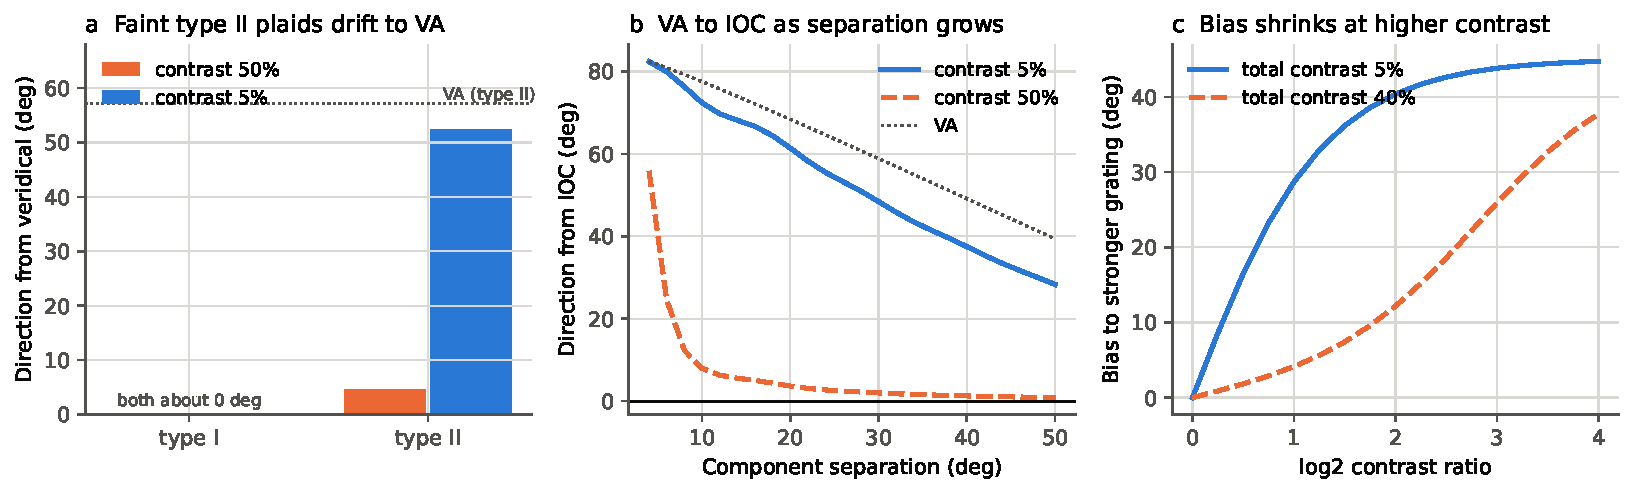
\includegraphics[width=\textwidth]{fig04_plaids.pdf}
\caption{Plaids: (a) type I vs II; (b) type II vs direction gap between gratings; (c) bias vs contrast ratio.}
\label{fig:plaids}
\end{figure*}
\subsection{Hypotheses and objectives}
I (i) rebuild the Weiss model and fit it to human data, (ii) derive an echo version of it, (iii) test it in a simulation of the bat experiment and (iv) compare it with the real bat data. The hypotheses, set at the mid-term, are:
\begin{itemize}[nosep]
\item H1: faint thin rhombuses look diagonal, fat ones do not.
\item H2: for a steady target, a line fit through the echoes beats aiming at the last echo.
\item H3: if the target changes speed while hidden, prediction can do worse.
\item H4: the slow prior helps only when echoes are very noisy.
\end{itemize}

\section{Methods}
\subsection{Model details}
\paragraph{Human model.} For an image sequence with space derivatives $I_x, I_y$ and time derivative $I_t$, Weiss et al.\ (Eq.~1) give
\begin{equation}
\mathbf{v}^* = -(A+\lambda I)^{-1}\mathbf{b},
\label{eq:weiss}
\end{equation}
\[
A=\begin{pmatrix}\sum I_x^2 & \sum I_xI_y\\ \sum I_xI_y & \sum I_y^2\end{pmatrix},\quad
\mathbf{b}=\begin{pmatrix}\sum I_xI_t\\ \sum I_yI_t\end{pmatrix},
\]
summed over the image. At lower contrast $A$ and $\mathbf{b}$ get smaller, so the prior pulls the estimate toward zero, most where the evidence is weakest.

\paragraph{Echo form (my derivation).} Echo $j$ gives target position $x_j$ at time $h_j$, with Gaussian noise $\sigma_e$. If the target moves on a line $x=a+v(h-\bar h)$, with a flat prior on $a$ and the slow prior $v\sim\mathcal{N}(0,\sigma_p^2)$, the most likely velocity is
\begin{equation}
v^*=\frac{\sum_j \tau_j d_j}{\sum_j \tau_j^2+\lambda},\qquad \lambda=\frac{\sigma_e^2}{\sigma_p^2},
\label{eq:echo}
\end{equation}
where $\tau_j=h_j-\bar h$ and $d_j=x_j-\bar x$. This is Eq.~\ref{eq:weiss} in one dimension, with $I_x\to\tau$ and $I_t\to-d$. The predicted position is $\bar x+v^*(t-\bar h)$, and its uncertainty grows the longer the target stays hidden. With $\lambda=0$ it is an ordinary line fit, which I use as the ablation.

\paragraph{Bat models.} As in Salles et al., every model points the head at $\arctan((s-1000)/300)$ for an estimated track position $s$ (mm), and can use only echoes that have already returned. The models are: (1) non-predictive: last echo position; (2) velocity estimation: last echo plus velocity (averaged over the last $k$ echoes) times the time since it; (3) predictive: model 2 plus a fixed angle; (4) mine: Eq.~\ref{eq:echo} through the last $k$ echoes; (5) mine with $\lambda=0$. On real data I add a fixed-head-angle model (model 1 plus a fixed angle) and allow a fixed angle in models 4 and 5.

\begin{figure*}[!tp]
\centering
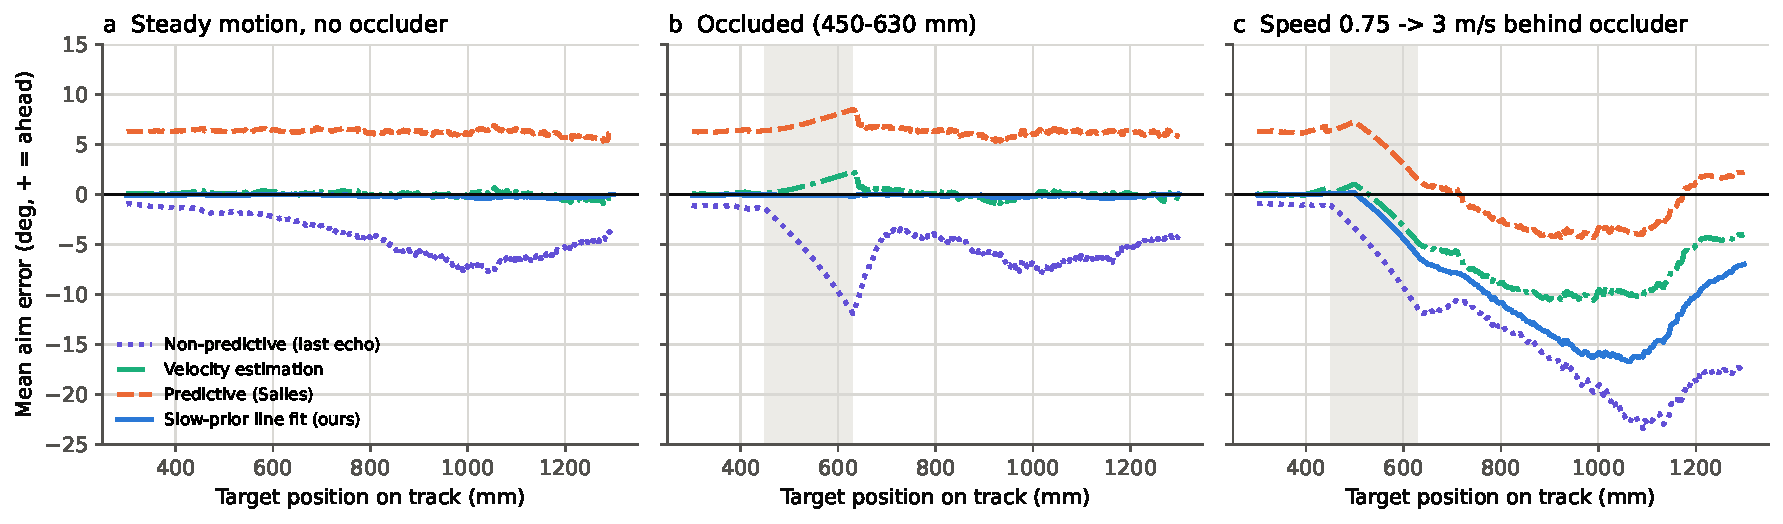
\includegraphics[width=\textwidth]{fig06_sim_error_over_time.pdf}
\caption{Simulated aim error along the track (mean of \simNTrialsCurves{} trials): (a) steady motion; (b) occluder at 450 to 630\,mm (grey); (c) speed-up behind the occluder. The Salles predictive model carries its fixed angle, fitted to bats, as error here.}
\label{fig:sim}
\end{figure*}
\begin{figure*}[!tp]
\centering
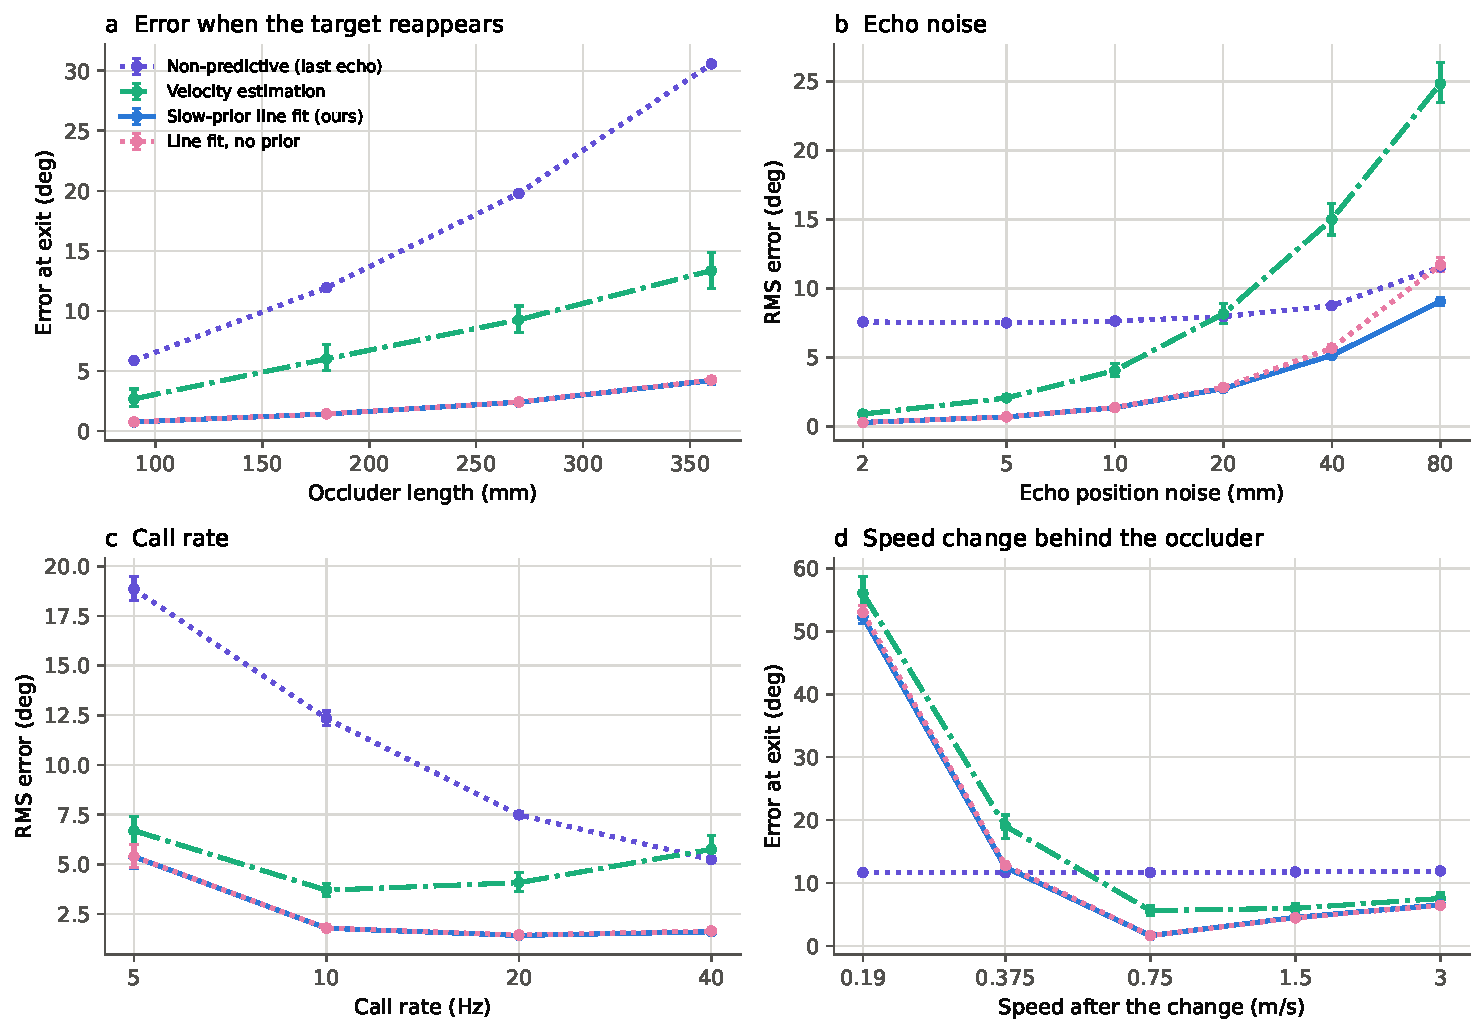
\includegraphics[width=0.85\textwidth]{fig07_sim_sweeps.pdf}
\caption{Sweeps (bootstrap 95\% CI): (a) occluder length, (b) echo noise, (c) call rate, (d) speed after a hidden change.}
\label{fig:sweeps}
\end{figure*}
\subsection{Implementation}
All code is plain NumPy; \texttt{scripts/run\_all.py} rebuilds every figure, video and number. Ten tests with known answers check the code, for example that the echo form gives the same result as the 1-D Weiss form.

\paragraph{Human stimuli and fit.} A soft-edged rhombus, gratings and plaids move 1 pixel per frame on a $128\times128$ grid. The paper gives no number for the rhombus angle, so I measured it from its drawings (thin = 40$^\circ$, fat = 10$^\circ$). Instead of setting $\lambda$ by hand per experiment, I used one rule, $\lambda=\kappa\,\mathrm{tr}(A)$ at full contrast with $\kappa=\humanKappa$. I read the six points of Weiss Fig.~4d (one subject) from the PDF, checked that the fit recovers known $\lambda$ values from simulated data, then fitted $\lambda$ by least squares with a bootstrap 95\% interval.

\paragraph{Bat data.} I ported the authors' trial selection and head-angle code from MATLAB \cite{sallesrepo} to Python and used their four bats: \realNBL{} standard and \realNOL{} occluded trials (paper: \paperNBL{} and \paperNOL), plus speed-change trials. The repository has no licence file, so I cite it and do not share the data. As in their code, RSS is the sum over 10\,ms bins of the squared mean offset (model minus head) in the 47 to 106\,cm window. The free settings ($k$, fixed angle, $\lambda$) were chosen by leaving one bat out: each bat was scored with settings fitted on the other three. Models were compared with paired Wilcoxon tests on per-trial RSS, with rank-biserial $r$ and Holm correction; the head lead was tested per 10\,ms bin with Bonferroni-corrected $t$-tests, as in the paper.

\paragraph{Simulation.} Simulated calls come at 20\,Hz with gamma-distributed intervals (fitted to the real calls), echo noise of \simBaseNoiseMm\,mm, $k=5$, $\sigma_p=1$\,m/s, and an occluder at 450 to 630\,mm. I varied occluder length, echo noise (2 to 80\,mm), call rate (5 to 40\,Hz) and the speed after a change (0.19 to 3\,m/s): \simNCells{} conditions, \simNTrialsPerCell{} trials each. The target counts as lost when the aim error is above \simTolDeg$^\circ$. Tests are paired (Wilcoxon, Holm).

\section{Results}
\subsection{Replication: does the model produce the human illusions?}
Yes, in direction. As contrast falls, the thin rhombus's direction swings toward the diagonal while the fat one stays near horizontal (Fig.~\ref{fig:human}a): at 100\% contrast the errors are \humanThinHighErr$^\circ$ and \humanFatHighErr$^\circ$, at 10\% \humanThinLowErr$^\circ$ and \humanFatLowErr$^\circ$. Making $\lambda$ ten times smaller or larger never swaps the order (H1 supported). Fainter gratings look slower (\humanGratingRelSpeedFortyAtTenth{} of true speed at one tenth contrast), but the result depends on absolute contrast, the same mismatch Weiss et al.\ report. Faint type II plaids move \humanPlaidTwoLowDir$^\circ$ off, close to the vector average (\humanPlaidTwoVA$^\circ$), while type I plaids move in the true direction (Fig.~\ref{fig:plaids}).


\begin{table*}[t]
\centering\small
\begin{tabular}{lcccc}
\toprule
Model & RSS, paper & RSS, mine & Held-out RSS & Fixed angle \\
\midrule
Non-predictive & \paperRssNonpredictive & \realRssNonpredictive & \realCvNonpredictive & n/a \\
Fixed head angle & \paperRssFixed & \realRssFixed & \realCvFixed & \realShiftFixed$^\circ$ \\
Velocity estimation & \paperRssVelocity & \realRssVelocity & \realCvVelocity & n/a \\
Predictive (Salles) & \paperRssPredictive & \realRssPredictive & \realCvPredictive & \realShiftPredictive$^\circ$ \\
Line fit, no prior & n/a & \realRssOursnoprior & \realCvOursnoprior & \realShiftOursnoprior$^\circ$ \\
Slow-prior line fit & n/a & \realRssOurs & \realCvOurs & \realShiftOurs$^\circ$ \\
\bottomrule
\end{tabular}
\caption{Fit to the standard trials (RSS in rad$^2$). Paper values from \cite{salles2020si}. Held-out: each bat scored with settings fitted on the other three, summed over bats.}
\label{tab:rss}
\end{table*}
\begin{figure*}[!tp]
\centering
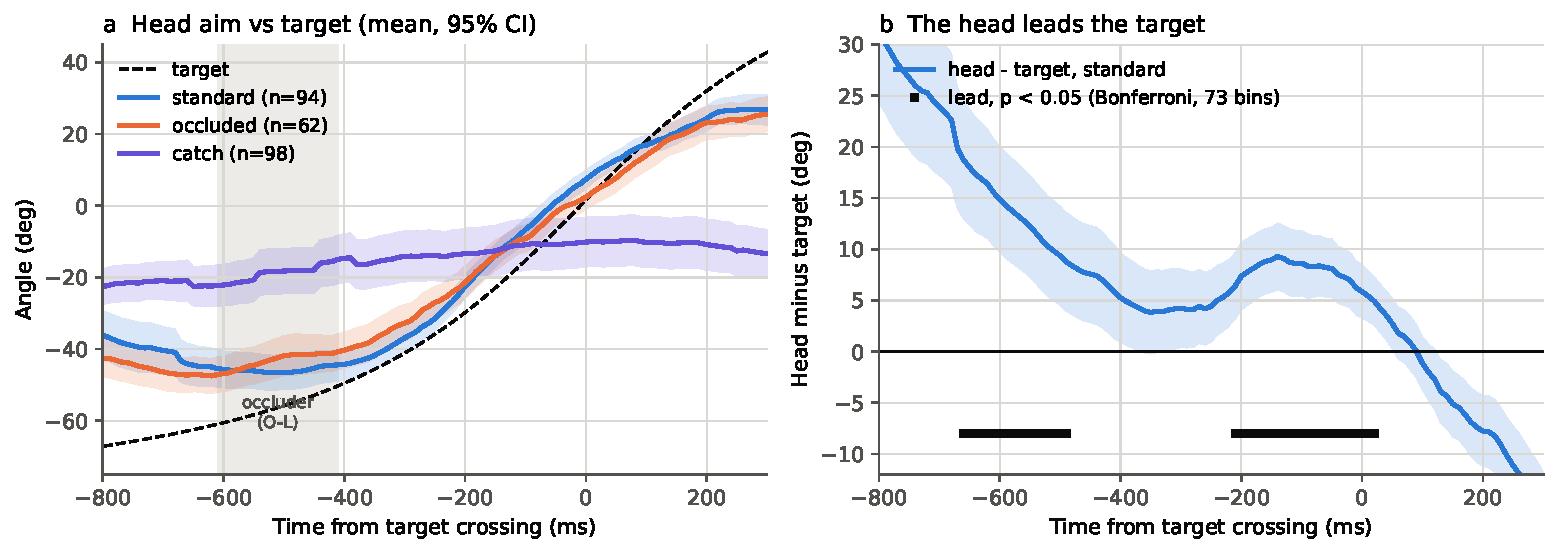
\includegraphics[width=\textwidth]{fig09_real_tracking.pdf}
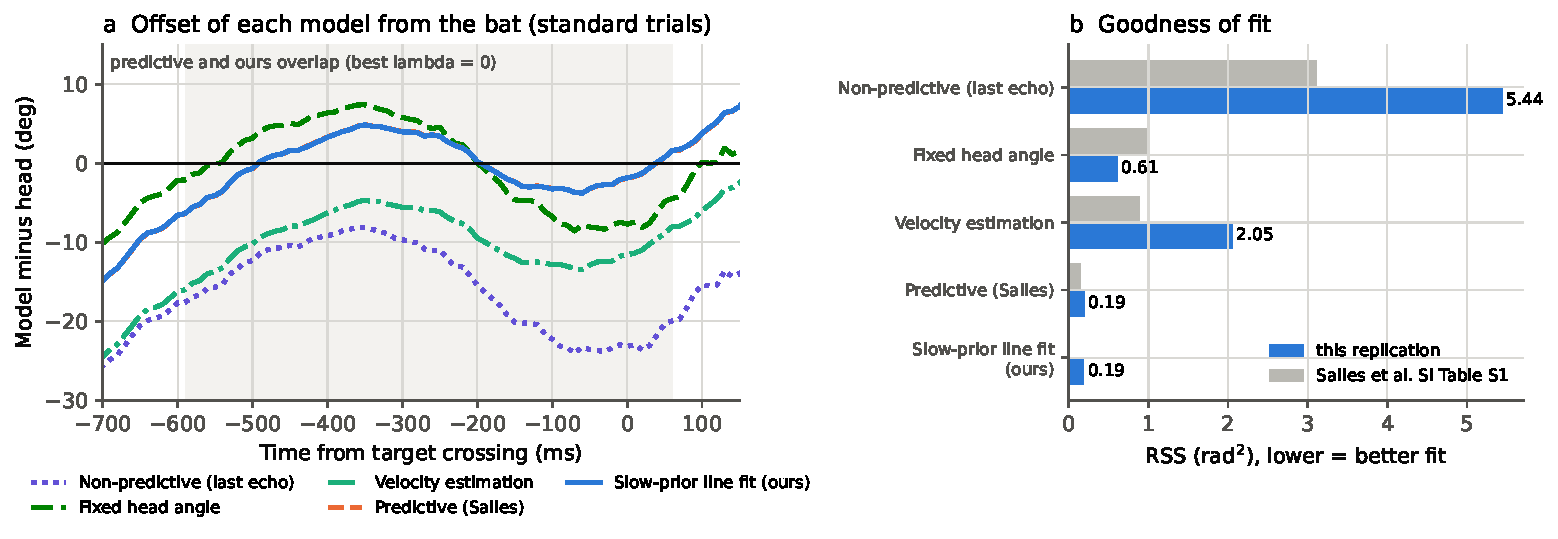
\includegraphics[width=\textwidth]{fig10_real_models.pdf}
\caption{Real bats \cite{sallesrepo}. Top: (a) mean head and target angle; (b) head minus target, bars: significant bins. Bottom: (a) model minus head; (b) RSS here and in the paper.}
\label{fig:real}
\end{figure*}
\subsection{Fit: does it match a human subject?}
Only the trend. Parameter recovery worked (error within \humanRecoveryMaxRelErr). On the six human points the best $\lambda$ was \humanLamFit{} (95\% interval \humanLamFitLo{} to \humanLamFitHi), RMSE \humanFitRMSE$^\circ$. The human curve rises sharply between 25$^\circ$ and 30$^\circ$; the model rises smoothly and is \humanFitMaxResid$^\circ$ too low at 30$^\circ$ (Fig.~\ref{fig:human}b).


\subsection{Extension: does the echo form follow a target in simulation?}
For a steady target, the line fit keeps the aim on the target (RMS \simSteadyRmsOurs$^\circ$), while aiming at the last echo lags (\simSteadyRmsNonpred$^\circ$; Holm $p=\simHTwoP$, $r=\simHTwoR$; Fig.~\ref{fig:sim}a). The last echo is off target for \simSteadyOffNonpred\,ms, the line fit for \simSteadyOffOurs\,ms (H2 supported). The lag of the last echo grows with occluder length: after 360\,mm hidden, its error when the target reappears is \simOcclThreeSixZeroExitNonpred$^\circ$, against \simOcclThreeSixZeroExitOurs$^\circ$ for the line fit (Fig.~\ref{fig:sweeps}a).

When the target slows from 0.75 to 0.19\,m/s while hidden, the line fit keeps the old speed: on reappearance its error is \simHiddenSlowExitOurs$^\circ$, against \simHiddenSlowExitNonpred$^\circ$ for the last echo ($p=\simHThreeSlowP$). When the target speeds up to 3\,m/s, prediction still wins (\simHiddenFastExitOurs$^\circ$ vs \simHiddenFastExitNonpred$^\circ$; Fig.~\ref{fig:sweeps}d). So H3 holds only for a slow-down (mixed).

The slow prior lowers the RMS error by only \simNoiseOneZeroGain$^\circ$ at 10\,mm echo noise and by \simNoiseEightZeroGain$^\circ$ at 80\,mm. The gain is significant only at \simPriorHelpsAt\,mm, and the prior never makes the error significantly worse (Fig.~\ref{fig:sweeps}b; H4 supported).



\subsection{Comparison: do real bats behave like the models?}
The bats' heads point ahead of the target (Fig.~\ref{fig:real}a), by \realLeadMeanDeg$^\circ$ on average ($t(\realLeadTrialDf)=\realLeadTrialT$, $p=\realLeadTrialP$; paper: $t(\paperLeadDf)=\paperLeadT$). In 10\,ms bins, \realLeadSigBins{} of \realLeadBins{} stay significant after correction; the paper reports all.

Models rebuilt from the real call times reproduce the main result of Salles et al.: prediction fits far better than the last echo (Table~\ref{tab:rss}, Fig.~\ref{fig:real}b). The replication is partial: my RSS values and fixed angles are larger, and the fixed-angle and velocity models swap order. Checking my code against the authors' MATLAB code did not find the cause.


The slow prior does not help. On all standard trials the best $\lambda$ was \realLamOurs, so my model becomes the plain line fit, which fits as well as the Salles predictive model (\realRssOurs{} vs \realRssPredictive). On held-out bats the prior made the fit worse than the predictive model (Holm $p=\realPOursVsPredictive$; Fig.~\ref{fig:lobo}), while the predictive model beat the last echo ($p=\realPPredictiveVsNonpredictive$). After a fast speed change behind the occluder, the last echo fits better than prediction (RSS \realChgOMFAfterNonpredictive{} vs \realChgOMFAfterPredictive), the real-bat version of H3.


\begin{figure}[t]
\centering
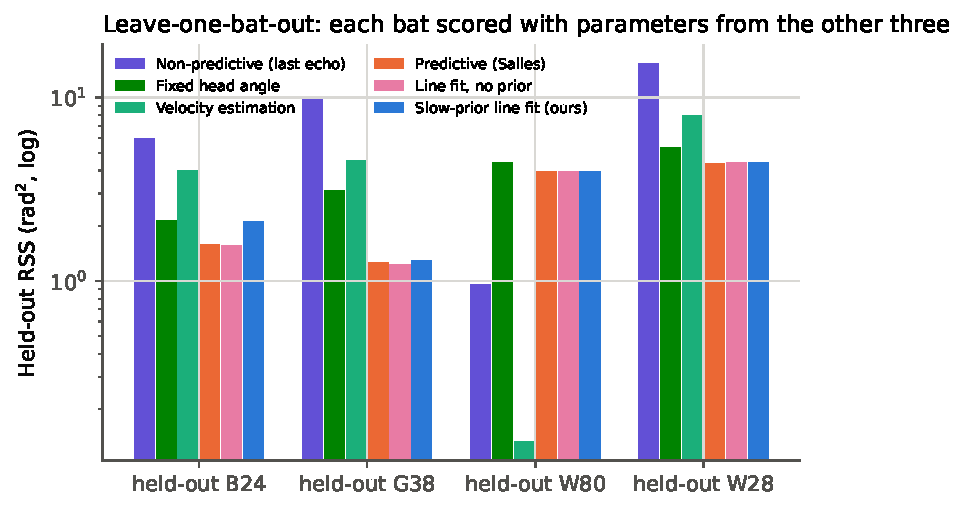
\includegraphics[width=\columnwidth]{fig11_lobo_cv.pdf}
\caption{Held-out RSS of each model per bat (log scale).}
\label{fig:lobo}
\end{figure}

\section{Discussion}
\paragraph{What the model explains.} One estimator with one parameter gives the right direction for every human illusion I tested. Its echo form predicts that bats combine several echoes and continue a hidden target's path; real bats lead the target and fit several-echo models best.

\paragraph{Where it fails.} The human model misses the sharp rise in the subject's curve, and its grating result depends on absolute contrast. For bats, the slow prior adds nothing. It pulls speed estimates toward zero and shortens the lead, while bats lead by more than any model without a fixed angle. A prior centred on zero is the wrong belief for a bat that expects prey to move, and the echoes here are too precise for any prior to matter much.

\paragraph{Alternative explanations.} For humans, Weiss et al.\ suggest contrast gain control: if contrast is first compressed, the same estimator fits the grating data much better, so slower percepts at low contrast may come from how contrast is coded rather than from the prior. For bats, a lead does not prove velocity estimation: a fixed angle added to the last echo already explains much of the head aim (Table~\ref{tab:rss}), and Salles et al.\ \cite{salles2021} describe a steering rule that needs no model of target motion. Prediction still beats the fixed angle on held-out bats (\realCvPredictive{} vs \realCvFixed), but the gap is small.

\paragraph{Limitations and future directions.} The human fit uses six points from one subject, the rhombus angle is my definition, the simulation assumes Gaussian noise, and the RSS replication is incomplete. Next: a prior centred on expected prey speed, echoes in angle and range, and fits for each bat.

\small
\bibliographystyle{unsrtnat}
\bibliography{refs}

\section*{Contribution statement}
This was a solo project by Deep Buha. I chose the topic, read the papers on motion perception and then on bat echolocation, and made the link between them, including the echo form of the Weiss equation (Eq.~\ref{eq:echo}). Claude Code (an AI assistant) wrote most of the code from my descriptions. I ran the simulations and experimented with the settings (such as $\lambda$, echo noise and call rate) to choose the ones reported here. I made the base simulations, and Claude Code refined them into the final videos. I wrote the report draft; Claude Code converted it to LaTeX, formatted it and suggested edits to the wording. The authors' bat data and MATLAB code \cite{sallesrepo} were used with attribution; the Python loader re-implements their trial selection.

\section*{AI use disclosure}
Before the mid-term I used Claude (claude.ai chat) to find papers and plan the project. For the end-term I used Claude Code (Claude Opus 5.5) to write the code, tests and figures from my descriptions, refine my base simulations into the final videos, build the slides, edit the presentation recording, and convert my report draft to LaTeX and format it. It checked its work with known-answer tests and against the authors' MATLAB code and published values. Every number in this report is produced by a script into \texttt{results/numbers.json}. I read through the report, slides and video and corrected the mistakes I found.

\end{document}
